% Figure 1: Slot ownership — one pacemaker cycle.
% Drop this into your .tex file where the ASCII placeholder is.
% Requires: \usepackage{tikz} in preamble.
%
% Slot I_s = [(11s+1)/110, (11s+10)/110], s = 1,...,9.
% x-coordinate system: 1 unit = 1/110 of cycle. Scale: x=0.115cm.
% Total width = 110 * 0.115cm = 12.65cm.

\begin{figure}[ht]
\centering
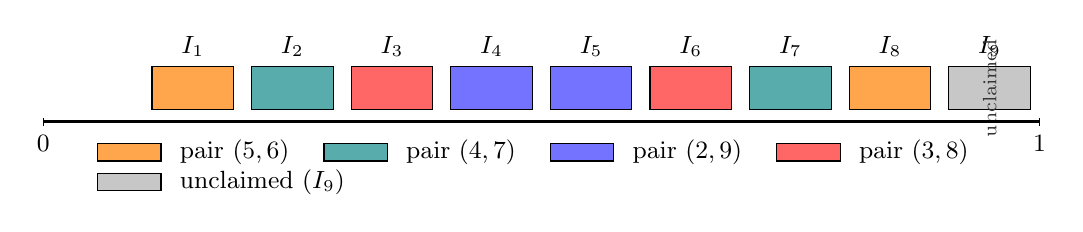
\begin{tikzpicture}[x=0.115cm, y=1cm]

  % --- Colour definitions (pair ownership) ---
  % Pair (2,9): blue   -> I_4, I_5
  % Pair (3,8): red    -> I_3, I_6
  % Pair (4,7): teal   -> I_2, I_7
  % Pair (5,6): orange -> I_1, I_8
  % Unclaimed:  grey   -> I_9

  \colorlet{pairA}{blue!55}      % (2,9)
  \colorlet{pairB}{red!60}       % (3,8)
  \colorlet{pairC}{teal!65}      % (4,7)
  \colorlet{pairD}{orange!70}    % (5,6)
  \colorlet{unclaimed}{black!22} % I_9

  % --- Slot rectangles (height 0.55) ---
  % I_1 [12,21]: pair (5,6) = pairD
  \fill[pairD]  (12,0) rectangle (21,0.55);
  % I_2 [23,32]: pair (4,7) = pairC
  \fill[pairC]  (23,0) rectangle (32,0.55);
  % I_3 [34,43]: pair (3,8) = pairB
  \fill[pairB]  (34,0) rectangle (43,0.55);
  % I_4 [45,54]: pair (2,9) = pairA
  \fill[pairA]  (45,0) rectangle (54,0.55);
  % I_5 [56,65]: pair (2,9) = pairA
  \fill[pairA]  (56,0) rectangle (65,0.55);
  % I_6 [67,76]: pair (3,8) = pairB
  \fill[pairB]  (67,0) rectangle (76,0.55);
  % I_7 [78,87]: pair (4,7) = pairC
  \fill[pairC]  (78,0) rectangle (87,0.55);
  % I_8 [89,98]: pair (5,6) = pairD
  \fill[pairD]  (89,0) rectangle (98,0.55);
  % I_9 [100,109]: unclaimed
  \fill[unclaimed] (100,0) rectangle (109,0.55);

  % --- Slot outlines ---
  \foreach \l/\r in {12/21,23/32,34/43,45/54,56/65,67/76,78/87,89/98,100/109}{
    \draw (\l,0) rectangle (\r,0.55);
  }

  % --- Slot labels above ---
  \foreach \s/\mid in {1/16.5, 2/27.5, 3/38.5, 4/49.5, 5/60.5,
                        6/71.5, 7/82.5, 8/93.5, 9/104.5}{
    \node[above, font=\small] at (\mid, 0.55) {$I_{\s}$};
  }

  % --- "unclaimed" label inside I_9 ---
  \node[font=\scriptsize, text=white!20!black, rotate=90] at (104.5,0.275)
        {unclaimed};

  % --- Timeline axis ---
  \draw[thick] (0,-0.15) -- (110,-0.15);
  \draw (0,-0.1) -- (0,-0.2)   node[below, font=\small] {$0$};
  \draw (110,-0.1) -- (110,-0.2) node[below, font=\small] {$1$};

  % --- Pair legend below timeline ---
  % Four coloured boxes with labels, centred under the figure.
  % y = -0.65 baseline for legend boxes (height 0.22).

  \def\bh{0.22}  % box height
  \def\bw{7}     % box width (in x-units)
  \def\ly{-0.65} % legend y

  % Space them evenly across [5,105] with gaps.
  % Positions chosen to sit roughly under each pair's two slots.
  % (2,9): centred near x=55
  % (3,8): centred near x=40 and x=72, average ~55 -> spread them out
  % Use fixed positions:
  %   pairD (5,6): x=10
  %   pairC (4,7): x=35
  %   pairA (2,9): x=60
  %   pairB (3,8): x=85

  \foreach \xpos/\col/\lbl in {
      6/pairD/{$(5,6)$},
     31/pairC/{$(4,7)$},
     56/pairA/{$(2,9)$},
     81/pairB/{$(3,8)$}}{
    \fill[\col] (\xpos,\ly) rectangle (\xpos+\bw, \ly+\bh);
    \draw       (\xpos,\ly) rectangle (\xpos+\bw, \ly+\bh);
    \node[right, font=\small] at (\xpos+\bw+1, \ly+0.5*\bh) {pair \lbl};
  }
  % Unclaimed swatch
  \fill[unclaimed] (6,\ly-0.38) rectangle (6+\bw, \ly-0.38+\bh);
  \draw            (6,\ly-0.38) rectangle (6+\bw, \ly-0.38+\bh);
  \node[right, font=\small] at (6+\bw+1, \ly-0.38+0.5*\bh) {unclaimed ($I_9$)};

\end{tikzpicture}
\caption{The four complementary pairs and their primary-slot assignments across one
pacemaker cycle. Each pair owns two non-adjacent slots (one in each half); the prime
modulus~$11$ forces this symmetric pairing. Slot~$I_9$ is unclaimed: no pair's
AP-limit witness labels correspond to it. Any completely blocking configuration must
assign some runner to cover $I_9$ off schedule, triggering the gap obstruction lemmas
of Section~5.}
\label{fig:slot-ownership}
\end{figure}
